% Do NOT change this "Section" title
% and do NOT add more "Section" level titles.
\section{Implementation}\label{sec:implementation}
Each component will be described in a dedicated section.

\subsection{Gripper}
The gripper have been designed in such a way that it is almost completely retracted in the tool compartment, providing a streamlined and hydrodynamic appearance of the robot. Naiad has two grippers installed on the underside of the hull. The gripper design can be seen in Figure \ref{fig:gripper}.

\begin{figure}[t]
    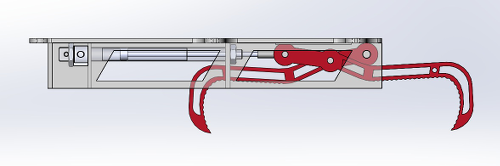
\includegraphics[width=0.5\textwidth]{./figure/gripper_open.png}
    \caption{Gripper at open position}
    \label{fig:gripper}
\end{figure}

In order to grip more effectively, they close with a very wide scooping motion, downwards and to the front. Moreover, the jaws are designed to interlock so they won't open accidentally. Each gripper is actuated by a single-acting naturally retracted cylinder, that in case of a power failure will open automatically (spring return), providing a "dead man's grip" mechanism.

\subsection{Marker}
The marker consists of a sphere attached to a tail ending in a conical shape pointing upwards. When inserted into the bay, this conical shape pushes and locks on a spring loaded latch. The latch is actuated by a single-acting, naturally retracted cylinder. There are two marker bays on the vessel. In Figure \ref{fig:marker}, the marker design is shown.

\begin{figure}[h]
    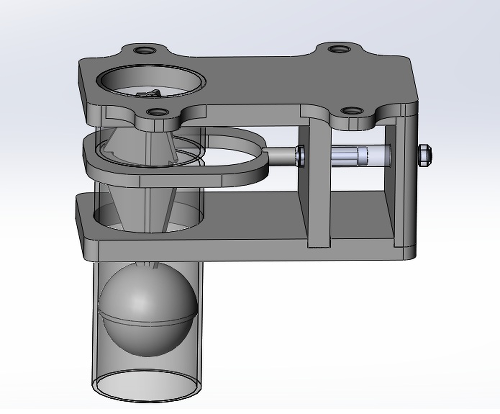
\includegraphics[width=0.5\textwidth]{./figure/marker_loaded.png}
    \caption{A loaded marker}
    \label{fig:marker}
\end{figure}

\subsection{Torpedo launcher}
There are two torpedo  bays on the front. The torpedoes have been designed to fit precisely into the bays and are kept in place by a small spring loaded ball. The torpedo design can be seen in Figure \ref{fig:torpedo}.

\begin{figure}[h]
    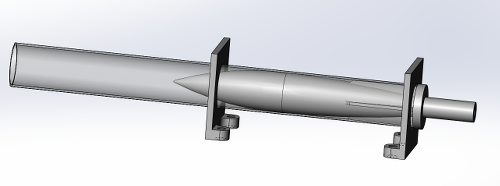
\includegraphics[width=0.5\textwidth]{./figure/torpedo_loaded.png}
    \caption{Torpedo in bay}
    \label{fig:torpedo}
\end{figure}

The torpedoes have slightly positive buoyancy in order to follow a linear trajectory. 

\subsection{Pneumatic System}
The system gas supply is a common 16gr CO2 cartridge. This cartridge is very small and also allows a rapid "recharge" simply by replacing it with a new one. Also, a larger or smaller cartridge can be inserted if required. An additional benefit is that as long as there is liquid CO2 evaporating inside the cartridge the output is relatively constant (depending on the gas temperature), whereas in a compressed air tank the pressure drops with every actuation in an exponential decaying manner.

\begin{figure}[h]
    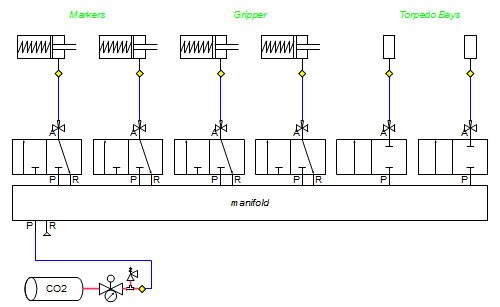
\includegraphics[width=0.5\textwidth]{./figure/pneumatics.png}
    \caption{Pneumatics system design}
    \label{fig:pneumatics}
\end{figure}

Leaving from the tank, the gas is passing through a regulator and supplied to a manifold, where it is distributed to the valves. A safety valve will protect the system and personnel from overpressure. The markers and the grippers will be actuated by four 3-way valves (one for each cylinder). Each torpedo bay will be actuated by a 2-way valve. On the output of all valves an adjustable needle valve regulates the flow rate, allowing to control the actuation speed. Quick-connect connectors will be used because of their simplicity and ease of set up. Polyurethane tubing will be preferred over other materials (eg. nylon), because it allows tight radius bends, something important in limited spaces. An overview of the pneumatic system design can be seen in Figure \ref{fig:pneumatics}.

\subsection{Pneumatics Controller}
A Generic CAN controller is used to control the pneumatic valves. The controller executes a control loop that starts by reading a received CAN message. This message can be a kill switch message, an execution mode message or a actuation message. Depending on the type, the appropriate dispatch procedure is called. The kill message dispatch procedure reads the payload of the message, and sets the controller to KILL state. Similarly, the mode message dispatch function sets the controller to the defined execution mode. Finally, the actuation message dispatch function energises the appropriate valve for the appropriate amount of time. Any message with undefined id or payload, is reject from the control loop. The actions of the controller for each can message can be seen at Table \ref{table:can_msg}.

\begin{table}
\centering
    \caption{Pneumatic controller input-output}
    \begin{tabular}{|c|c|c|c|} \hline
    \label{table:can_msg}
	\textbf{id} & \textbf{payload} & \textbf{action} & \textbf{out} \\ \hline
        KILL & KILL & kill enabled & n\\ \hline
        KILL & not KILL & kill disabled & n \\ \hline
        KILL & other & - & n \\ \hline
        MODE & SIMULATE & sim enabled & n \\ \hline
		MODE & not SIMULATE & sim disabled & n \\ \hline
		MODE & other & - & n \\ \hline
		ACTUATE & VALVE & actuate valve & y \\ \hline
		ACTUATE & other & - & n \\ \hline
		other & other & - & n \\ \hline
    \end{tabular}
\end{table}